% Paper 9 (TN Holdings), DRAFT 2, home, 2026-11-14 (owner: release 16 November; the light-cone work in paper 9,
% reframed as "what sets r"; the post-hoc rescaling as a problem statement only). Built from notes/paper9/part_a_from_paper8.tex, part_a_depth_draft.tex,
% part_b_draft.tex (workplace, numbers checked there against each record's scores.json), the r-thread
% (notes/paper9/r_thread_2026-11-13), the twin test (results/twin-2026-11-13), the yardstick
% (notes/paper9_yardstick) and the XX size test (notes/xxsize_2026-11-14). Every number is quoted from the committed
% record named beside it. Figures: notes/paper9/figures.py; rescaling: notes/paper9_posthoc/rescale.py.
\documentclass[10pt,a4paper]{article}
\usepackage[margin=2.2cm]{geometry}
\usepackage{amsmath,amssymb}
\usepackage{booktabs}
\usepackage{graphicx}
\usepackage[hidelinks]{hyperref}
\usepackage{url}
\setlength{\parskip}{4pt}
\setlength{\parindent}{0pt}
\sloppy
\newcommand{\pending}[1]{\textbf{[PENDING: #1]}}

\title{What Makes Raw Quantum Dynamics Readable?\\ The Share of Signal Kept, Across 179 Results on IBM Heron}
\author{TN Holdings\\ \small contact: \texttt{love.os.architect@proton.me}}
\date{16 November 2026}

\begin{document}
\maketitle

\begin{abstract}
Papers 7 and 8 of this series ran user-written circuits on IBM Heron devices through an operating layer (psf-os) that
places a circuit from the coupling graph and the failed elements only, adds its own controls to each job and applies
no error mitigation; a result \emph{reads} when its mean squared error is at most half the mean square of the exact
answer. This paper asks what decides whether a raw result reads. We split the error exactly as
$\mathrm{MSE}/\overline{e^2} = (1-r)^2 + \text{rest}$, with $r = \sum ze/\sum e^2$ the share of the exact pattern the
device keeps. Since the rest is never negative, $r < 1 - 1/\sqrt2 \approx 0.293$ means ``does not read'' by
construction; the measured statement is the converse. Across every result of the series with an exact answer (179),
including four of IBM's 2023 utility observables run raw (reading to 8 steps for $\langle Z_{106}\rangle$) and the 1D
Fermi--Hubbard model at $U = 4$ (reading at every size from 40 to 120 qubits at 4 Trotter steps, at none at 6), 160 of
the 166 results with $r \ge 0.293$ read; the six that did not have a wrong shape as large as the shrink, or sit at the
line. So whether a result reads is mostly whether $r$ stays above 0.293, and the question becomes what sets $r$.
A declared test on two devices found that it is not the CZ depth alone: at equal depth an 81-qubit XX chain kept less
than a 33-qubit one, by up to 0.18. Where the 33-qubit chain is the first 33 qubits of the 81-qubit one, the extra loss
on the same qubits opens next to where the longer chain continues and moves inward with depth; a repeat in a new job
gave the same order, while a simulation with uniform local noise gives no gap. Finally, we state a problem rather than a
method: dividing raw values by a measured share (of a full-signal circuit, or of a Clifford twin with the same pulses)
cannot undo what is not a shrink, and on our records it changed few verdicts and made some results worse. No quantum
advantage is claimed: every answer is computed exactly on a classical machine.
\end{abstract}

\section{Introduction}\label{sec:intro}
Paper 7 (doi:10.5281/zenodo.24046673) and paper 8 (doi:10.5281/zenodo.24136512) reported raw device results under
one policy: placement from the coupling graph and the failed elements only, the device chosen by its queue, the job's
own controls (floor, mirror, ring sentinel) in the same submission, no mitigation, dynamical decoupling and twirling
off, answers sealed by hash before each run, every declaration pushed to git before the device record of its run was
fetched. Within one family the boundary of reading lies along depth, but different families stop at very different
depths. This paper asks three questions.
\begin{itemize}
\item Is there one quantity that tells, for every result with an exact answer, whether it reads? We find the kept
share $r$, with a line at 0.293 that comes from an identity, and test how often being above the line is enough
(sections~\ref{sec:measures}--\ref{sec:yardstick}), on all results so far, including two targets the field uses as
references: IBM's 2023 utility observables (Kim et al.\ 2023) and the 1D Fermi--Hubbard model past exact
diagonalisation (sections~\ref{sec:utility}, \ref{sec:hubbard}).
\item What sets $r$? Depth, the size of the signal, the size of the circuit, the qubits used
(sections~\ref{sec:size}, \ref{sec:cone}).
\item If the loss were a pure shrink, dividing by $r$ would undo it. What remains when a user divides by a share they
can measure (section~\ref{sec:posthoc})?
\end{itemize}
Not claimed: quantum advantage; that any mitigation does or does not work (none is used, and section~\ref{sec:posthoc}
is not a mitigation method); anything about devices, days or families not run. Most results are one device and one
day; each section says which.

\section{Measures}\label{sec:measures}
For a circuit with exact values $e_i$ and raw device values $z_i$ (expectation values over its measured qubits or
points), the declared verdict is
\[ \textsc{reads} \iff \mathrm{MSE} = \overline{(z-e)^2} \le \tfrac12\,\overline{e^2}, \]
i.e.\ the device's error is at most half of what the all-zero guess would make. Beside it we report
\[ r = \frac{\sum_i z_i e_i}{\sum_i e_i^2}, \qquad
   \frac{\mathrm{MSE}}{\overline{e^2}} = (1 - r)^2 + \underbrace{\frac{\overline{(z - r e)^2}}{\overline{e^2}}}_{\text{rest}}. \]
The split is an identity ($r$ is the least-squares scale, so the cross term vanishes). $r$ is the share of the exact
pattern the device keeps; the rest is everything that is not a uniform shrink (a wrong shape, offsets, shot noise).
Two consequences follow without data. If the device only shrank the signal ($z = re$), \textsc{reads} would hold exactly
when $r \ge 1 - 1/\sqrt2 \approx 0.293$, whatever the size of the signal. Because the rest is never negative,
$r < 0.293$ always means ``does not read''. What a device record can show is how often $r \ge 0.293$ is enough, and how
far above the floor $(1-r)^2$ each result sits (figure~\ref{fig:yardstick}).

\section{IBM's 2023 utility observables, raw}\label{sec:utility}
\subsection{The run of 10 November}
\texttt{results/utility-2026-11-10}. Kim et al.\ (2023) ran a kicked Ising circuit on ibm\_kyiv (Eagle, 127 qubits)
and reported error-mitigated values; here four of their observables were run raw, with the published circuit on the
published graph. Eagle's graph embeds in Heron r2's in two ways. All $R_{ZZ}$ commute, so after $t$ steps an
observable depends only on the gates within $t$ edges of its support; per observable, the first embedding whose light
cone holds no failed element was used, the gates on failed elements (outside the cone) were left out, and the
observable's exact value is the published circuit's. Exact values came from a tensor-network contraction of the
light-cone network, computed twice independently (agreement $2\times10^{-15}$) and checked against the stabilizer
method on all 127 qubits at $\theta_h = 0$ and $\pi/2$; they were sealed before the run.

On ibm\_fez (ibm\_marrakesh had no clear cone for any observable), 17 values of $\theta_h$, 4000 shots:
$\langle Z_{106}\rangle$ after 4 steps (564 CZ) reads; the weight-10 product after 5 steps (705 CZ) reads and keeps 0.61
of its exact $+1$ at $\theta_h = \pi/2$; the weight-17 product and the Fig.~4a product (690 CZ) do not read: at
$\theta_h = \pi/2$ they keep their sign and 7 to 9\% of the exact $-1$. Each product's own mirror falls the same way
(parity 0.50, 0.12, about 0). No comparison is made with IBM's mitigated values.

\subsection{How deep the observables read (11 November)}\label{sec:utility-depth}
\texttt{results/utility-depth-2026-11-11}, ibm\_fez (ibm\_marrakesh placed no clear cone),
prereg/utility\_depth\_2026-11-11.md. The exact values were extended past the 11-10 depths by the same light-cone
contraction (checked at the Clifford points against the stabilizer method on all 127 qubits) and sealed before the
run. One job of 137 circuits, 17 values of $\theta_h$ per observable:

\begin{center}\small
\begin{tabular}{lrrrcc}
\toprule
observable & steps & CZ & light cone (qubits) & MSE / mean square & AGREES (of 17) \\
\midrule
$Z_{106}$ & 4 & 564 & 17 & 0.0198 / 0.4145 reads & 7 \\
$Z_{106}$ & 5 & 705 & 25 & 0.0149 / 0.4073 reads & 7 \\
$Z_{106}$ & 6 & 846 & 31 & 0.0117 / 0.4005 reads & 8 \\
$Z_{106}$ & 7 & 987 & 38 & 0.0110 / 0.3968 reads & 8 \\
$Z_{106}$ & 8 & 1128 & 43 & 0.0108 / 0.3921 reads & 8 \\
weight-10 & 5 & 705 & 37 & 0.0238 / 0.1672 reads & 11 \\
weight-10 & 6 & 846 & 42 & 0.0005 / 0.0038 reads & 17 \\
\bottomrule
\end{tabular}
\end{center}

The prediction that weight-10 would not read at 6 steps failed. Both readings need care. The exact $Z_{106}$ curve
changes little with depth (the 4- and 8-step curves differ by at most 0.11), and its MSE falls with depth because the
device's tail at large $\theta_h$ shrinks: this is reading a slowly changing answer. Weight-10 at 6 steps is a small
signal (mean square 0.0038): the verdict is given as declared. Against 11-10 on the same device and circuits,
$Z_{106}$ at 4 steps had MSE 0.0198 (0.0207) and weight-10 at 5 steps 0.0238 (0.0226).

\section{The one-dimensional Fermi--Hubbard model, raw}\label{sec:hubbard}
\subsection{Circuit, ruler and classical check}
$L$ sites on $2L$ qubits in the interleaved Jordan--Wigner order, N\'eel start, $J = 1$, first-order Trotter steps of
$dt = 0.25$: onsite $R_{ZZ}(U\,dt/2)$ and $R_Z(-U\,dt/2)$, then even and odd bonds by fermionic swaps and $XX+YY$
hopping; checked against the fermion operators ($5.6\times10^{-16}$ at $L = 3$); $10L-8$ CZ and 12 CZ layers per step
on a line, no routing. At $U = 0$ the circuit is free fermions, exact at any size from a $2L\times2L$ single-particle
matrix: the \emph{ruler}, run in the same job on the same chain, with the same CZ count and depth as $U = 4$ (each
onsite $R_{ZZ}$ written as two cancelling CZ). The $U = 4$ answers come from matrix-product states; before any device
run a check with a criterion fixed beforehand covered $L = 20$, 24, 30 at 4, 6, 8 steps (untruncated against truncated
MPS, $2.5\times10^{-8}$ and $7.8\times10^{-8}$; at 8 steps bond dimensions 1024 and 2048 within $8\times10^{-10}$).

\subsection{40 to 120 qubits}
\texttt{results/hubbard-2026-11-11} and \texttt{hubbard-big-2026-11-11}, ibm\_fez, 4000 shots, answers sealed:

\begin{center}\small
\begin{tabular}{rrrrcc}
\toprule
$L$ (qubits) & steps & CZ & CZ per qubit & $U=4$: MSE / mean square & ruler: MSE / mean square \\
\midrule
20 (40) & 2 & 384 & 9.6 & 0.0094 / 0.1814 reads & 0.0063 / 0.0824 reads \\
20 (40) & 4 & 768 & 19.2 & 0.0080 / 0.0460 reads & 0.0395 / 0.1316 reads \\
20 (40) & 6 & 1152 & 28.8 & 0.0141 / 0.0219 does not read & 0.0480 / 0.0512 does not read \\
30 (60) & 2 & 584 & 9.7 & 0.0093 / 0.1725 reads & 0.0043 / 0.0742 reads \\
30 (60) & 4 & 1168 & 19.5 & 0.0068 / 0.0375 reads & 0.0422 / 0.1312 reads \\
30 (60) & 6 & 1752 & 29.2 & 0.0125 / 0.0176 does not read & 0.0361 / 0.0452 does not read \\
45 (90) & 2 & 884 & 9.8 & 0.0191 / 0.1672 reads & 0.0110 / 0.0697 reads \\
45 (90) & 4 & 1768 & 19.6 & 0.0101 / 0.0325 reads & 0.0324 / 0.1383 reads \\
60 (120) & 2 & 1184 & 9.9 & 0.0132 / 0.1637 reads & 0.0062 / 0.0661 reads \\
60 (120) & 4 & 2368 & 19.7 & 0.0073 / 0.0290 reads & 0.0307 / 0.1308 reads \\
\bottomrule
\end{tabular}
\end{center}

Every size from 40 to 120 qubits read at 2 and 4 steps (48 CZ layers at 4); neither size run at 6 steps (72 layers)
read. The predictions that $U = 4$ would read at 6 steps and that the ruler would keep the same share as $U = 4$ (ratio
$r(U4)/r(U0)$ within 0.9--1.1) failed: the ratio held at 2 steps (0.90--0.94) and not at 4 or 6 (1.00--3.40). The
ruler's exact pattern spreads ballistically while the $U = 4$ N\'eel pattern decays slowly, so the two arms carry
different signals; the ruler stayed beside the verdicts and corrected nothing. The exactly-zero site charge
$\langle Z_{i\uparrow}\rangle + \langle Z_{i\downarrow}\rangle$ read 0.05--0.10 on average.

\subsection{One time, two step sizes}
\texttt{results/hub-dt-2026-11-12}, ibm\_fez. At $L = 20$, the same time in two step sizes, each arm against its own
circuit's answers (all four read) and, as declared, against the continuum limit: at $Jt = 1$ the 2-step circuit was
closer than the 4-step one by 0.0009 in MSE (1.7 shot standard errors); at $Jt = 0.5$ the 2-step circuit was closer
than the 1-step one by 0.0172 (17 standard errors), the 1-step circuit's Trotter error (0.0164) being larger than the
2-step circuit's whole device error.

\section{One yardstick for every result}\label{sec:yardstick}
\subsection{The table}
\texttt{notes/paper9\_yardstick/line\_all.py} collects every recorded result of the series with an exact answer and a
declared verdict (written after all were scored): XX chains (75 circuits: the 91-qubit depth scan of 11-12, the size
test and its repeat of 11-14, the twin test of 11-13), Hubbard (31: section~\ref{sec:hubbard} with both arms, the twin
test), IBM 2023 utility (11 observable-depth units, over their $\theta_h$ points), 3D kicked Ising (48 arms of 11-10,
paper 8), the daily record (11 problems, 2026-11-05 to 11-14) and the dual-unitary curves at 51, 71 and 91 qubits (3,
papers 7 and 8).

\begin{center}\small
\begin{tabular}{lrrr}
\toprule
family & results & read & $r \ge 0.293$ gives the verdict \\
\midrule
XX chain & 75 & 63 & 72 \\
Hubbard (both arms, two step sizes) & 31 & 26 & 28 \\
IBM 2023 utility & 11 & 9 & 11 \\
3D kicked Ising & 48 & 48 & 48 \\
daily record (P4 chain) & 11 & 11 & 11 \\
dual-unitary curves & 3 & 3 & 3 \\
\midrule
all & 179 & 160 & 173 \\
\bottomrule
\end{tabular}
\qquad
\begin{tabular}{lrr}
\toprule
 & reads & does not read \\
\midrule
$r \ge 0.293$ & 160 & 6 \\
$r < 0.293$ & 0 & 13 \\
\bottomrule
\end{tabular}
\end{center}

Of the 13 results with $r < 0.293$, none read (the identity). Of the 166 with $r \ge 0.293$, 160 read (96\%). Every
result that read has $r \ge 0.293$; of the 19 that did not, $r$ alone flags 13. The six it misses:
\begin{itemize}
\item Hubbard at 6 steps, three times ($L = 20$ and 30 on 11-11; $L = 20$ on 11-13): $r$ = 0.38--0.51, but the rest is
0.27--0.32, as large as the shrink. The device keeps much of the pattern and gets its shape wrong.
\item The XX chain at the line itself, three times (MSE / mean square 0.504--0.518, rest 0.03--0.06).
\end{itemize}
Where the error is mostly a shrink (the XX chain, the utility products of weight 10 and 17, the 3D Ising arms), $r$ alone
tells the verdict. Where half the error is rest at every depth (Hubbard at $U = 4$: rest 0.49--0.52 of the ratio), the
line in $r$ sits higher than 0.293 and the boundary comes earlier than $r$ says. Only the 20 cells of
section~\ref{sec:size} tested the line under a declaration (20 of 20); the rest of the table is an after-the-fact
collection.

\begin{figure}[t]
\centering
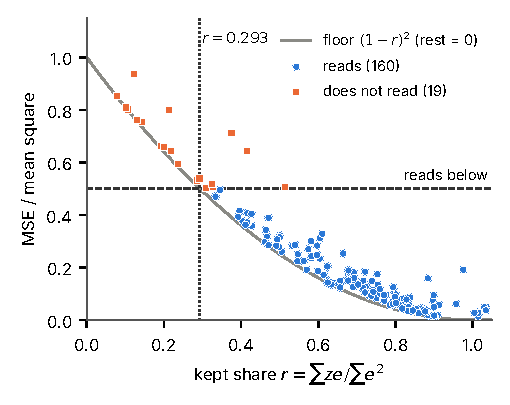
\includegraphics[width=0.55\linewidth]{fig_yardstick.pdf}
\caption{MSE / mean square against the kept share $r$ for the 179 results. No point can lie below the floor
$(1-r)^2$ (rest = 0); a result reads below the dashed line. Left of $r = 0.293$ nothing reads; right of it, the six
that do not are Hubbard at 6 steps (well above the floor: a wrong shape) and three XX circuits at the line.}
\label{fig:yardstick}
\end{figure}

\subsection{Seeing $r$ before the verdict: the Clifford twin}\label{sec:twin}
\texttt{results/twin-2026-11-13}, ibm\_marrakesh, prereg/twin\_2026-11-13.md. On Heron, $R_Z$ is a frame change with no
pulse; rounding every $R_Z$ of a compiled circuit to a multiple of $\pi/2$ gives a circuit with the same pulses (same
CZ, same $\sqrt X$, same timing) whose exact answer a stabilizer simulation gives at any size (psf-os, \texttt{twin}).
Run beside the user's circuit in the same job, its own $r$ is a direct, mitigation-free reading of how much signal the
device keeps on that pulse sequence. On the XX chain at 91 qubits (4, 8, 12 steps) and Hubbard at $L = 20$ (2, 4, 6
steps): $r_{\text{twin}} - r$ = +0.017, +0.018, +0.007 and $-0.051$, $-0.047$, +0.039. The declared bound 0.05 failed
narrowly (Hubbard at 2 steps). ``$r_{\text{twin}} \ge 0.293$'' matched the user circuit's verdict in 5 of 6; the miss is
Hubbard at 6 steps, the same shape error as above, which a twin cannot see.

\section{What sets $r$: depth, angle and size}\label{sec:size}
\texttt{notes/xxsize\_2026-11-14}, prereg/xxsize\_2026-11-14.md, results \texttt{xxsize-2026-11-14-marrakesh} and
\texttt{-fez}. On 11-12 (ibm\_fez, 91 qubits) $r$ was nearly the same at $\theta = \pi/4$ and $\pi/2$ at every depth,
which suggested that $r$ depends on the CZ layers a qubit goes through and not on the circuit's size or signal. A
declared test on ibm\_fez and ibm\_marrakesh: XX+YY brickwork chains of 33 and 81 qubits, N\'eel start, both angles,
8 to 64 CZ layers (the same layers at both angles), one job per size and device, free-fermion answers sealed by hash.
\begin{itemize}
\item angle: $|r(\pi/4) - r(\pi/2)| \le 0.05$ in 12 of 20 pairs (largest 0.074) --- failed;
\item size: $|r(81) - r(33)| \le 0.05$ in 7 of 20 pairs; $r$ lower at 81 qubits in all 20, by up to 0.18 on ibm\_fez ---
failed;
\item ``$r \ge 0.293$'' matched the verdict in 20 of 20 --- held. Readable depth at $\pi/4$: ibm\_marrakesh 64 layers at both
sizes; ibm\_fez 64 at 33 qubits and 32 at 81.
\end{itemize}
Beside (not judged): fits $r = A\,e^{-L/\lambda}$ over the CZ layers $L$ give $\lambda$ = 78 layers on ibm\_marrakesh
and 43 on ibm\_fez with both sizes pooled, equal to the 91-qubit values of 11-13 and 11-12, but 88 and 71 (marrakesh)
and 57 and 35 (fez) per size: the pooled agreement is not by itself evidence that a device's decay length is the same
from day to day. So $r$ is the share kept by \emph{this} circuit on \emph{these} qubits today, not a property of depth
alone (figure~\ref{fig:size}).

\begin{figure}[t]
\centering
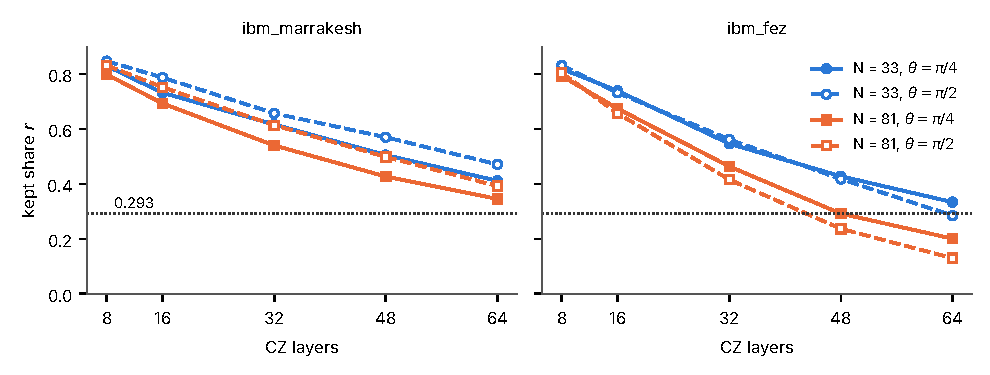
\includegraphics[width=\linewidth]{fig_size.pdf}
\caption{Kept share $r$ of the XX chain against CZ layers, 33 and 81 qubits, $\theta = \pi/4$ (filled) and $\pi/2$
(open), 14 November 2026. At equal layers the 81-qubit chain keeps less on both devices. Dotted: $r = 0.293$.}
\label{fig:size}
\end{figure}

\section{Where the extra loss appears: along the chain}\label{sec:cone}
\subsection{The same qubits inside a shorter and a longer circuit}
On ibm\_marrakesh the 33-qubit chain was exactly the first 33 qubits of the 81-qubit chain, in the same order, so the
same qubits can be compared inside the two circuits. After the verdicts (exploratory, \texttt{split.py}): at $\pi/4$,
on the 33 shared qubits $r$ = 0.617 in the short circuit and 0.558 in the long one at 32 layers, 0.411 and 0.343 at 64;
in the long circuit, its 48 other qubits kept about as much as the shared ones (0.527 and 0.347). The added qubits are
not simply worse; the shared ones lose more when the chain goes on. Split by position (blocks of 11 qubits: \emph{far}
from where the long chain continues, \emph{mid}, \emph{near}), the gap $g = r_{33} - r_{81}$ opened in the near block
first and moved inward with depth; at $\pi/2$, the fastest-spreading case, it reached the far block only at 48--64
layers.

\subsection{A repeat in a new job (declared after seeing the first run)}
\texttt{prereg/xxcone\_2026-11-14.md}, \texttt{results/xxcone-2026-11-14}. The same two jobs were run again on
ibm\_marrakesh 34 minutes later (13:04 CET), with three predictions chosen after seeing the first run and holding on
it; this tests whether the pattern comes back, not a first test. The analysis (\texttt{cone.py}) was fixed before the
run. (1) $\pi/4$, far block, $|g| \le 0.03$ at all five depths: failed by one cell (48 layers, +0.061; the others
+0.007 to +0.021). (2) $\pi/4$ at 16 and 32 layers, $g_{\text{near}} - g_{\text{far}} \ge 0.05$: held (+0.098,
+0.168). (3) $\pi/2$, far block, $|g| \le 0.03$ up to 32 layers and $g \ge 0.03$ at 64: held ($-0.005$, +0.007, +0.002;
+0.108). The order in which the gap opens came back: near first, mid from 32 layers, far last (figure~\ref{fig:gap}).

\begin{figure}[t]
\centering
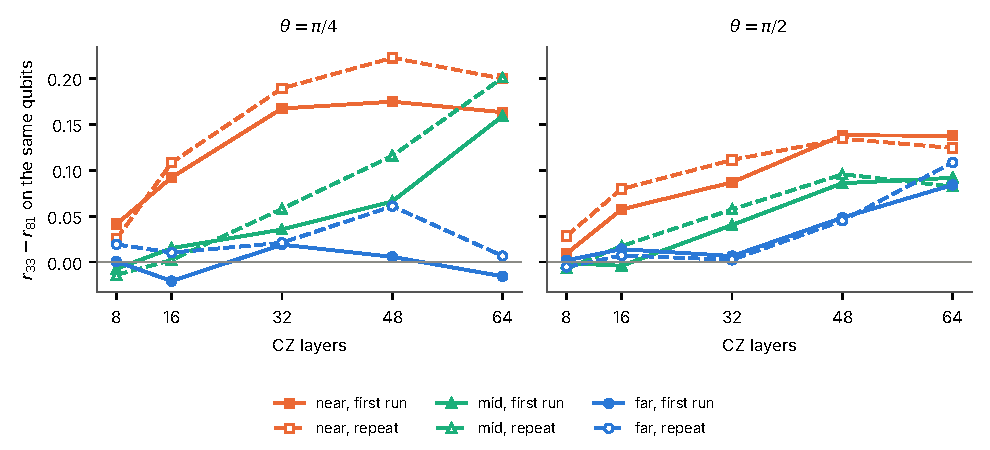
\includegraphics[width=\linewidth]{fig_gap.pdf}
\caption{Gap $r_{33} - r_{81}$ on the same 33 qubits of ibm\_marrakesh, by block of 11 qubits (near: next to where the
81-qubit chain continues), first run (12:30 CET, filled) and repeat (13:04 CET, open), 14 November 2026.}
\label{fig:gap}
\end{figure}

\subsection{What it is not: uniform noise}
A first reading was a light cone: errors spread with the dynamics, so a qubit's shrink would count the errors inside
its light cone, which the short chain cuts off at its end. A desk check does not support that form. A stabilizer
simulation (stim) of the recorded $\theta = \pi/2$ circuits of the repeat with one uniform local noise model (CZ
depolarising 0.003, single-qubit 0.0003, readout 0.015; nothing taken from the device) gives a gap within $\pm0.004$ in
every block at every depth, against up to +0.13 on the device. In this circuit a measured $Z$ follows its particle's
path, and uniform noise puts the same number of errors on a path whether the chain is 33 or 81 long. An illustration,
not a fit: tripling the CZ error on couplers that touch the extension (positions 33--80) gives a gap that grows with
depth and moves inward (far block +0.024 only at 64 layers), as on the device, but in a different order (mid above near
from 16 layers; on the device near first). The device gap therefore needs elements that differ along the paths the
dynamics takes; which elements, and how, is not measured here (the calibration is not read). Our own readout record of
the extension qubits has a heavier tail (mean $1 - z(|0\rangle)$ 0.039 against 0.020), but readout acts at the end of a
path and does not explain the gap alone.

For the yardstick this has a plain consequence: a result's $r$ depends on where its circuit sits and how far its
dynamics reaches on the device that day, so $r$ measured on one circuit is not $r$ for another of the same depth.

\section{Undoing the shrink after the fact: a problem statement}\label{sec:posthoc}
If the device's error were a pure shrink, $z = re$, dividing by $r$ would restore the answer. We state what that idea
meets on our records, computed beside the results and never used for any verdict (\texttt{notes/paper9\_posthoc/rescale.py}).
Dividing by a scale $s$ gives
\[ \frac{\overline{(z/s - e)^2}}{\overline{e^2}} = \frac{\text{rest} + (r - s)^2}{s^2}, \]
so even the best single scale ($s = r$) leaves $\text{rest}/r^2$: the part that is not a shrink, enlarged by $1/r^2$,
shot noise included.
\begin{itemize}
\item \emph{Oracle} ($s = r$, taken from the exact answer itself, which a user does not have): of the 179 results, 170
would read instead of 160 (11 gained, with $r$ from 0.077 to 0.327; 1 lost, an XX result that read at 0.496 and gives
0.562 after); the ratio grows for 26. Nine still do not read, among them Hubbard at 6 steps ($\text{rest}/r^2$ = 1.0 to
11.2): a wrong shape is not a scale.
\item \emph{Full-signal ruler} (the $\pi/2$ circuit of the same chain, depth and job, a Clifford circuit with the same
gates): over the 30 $\pi/4$ circuits of section~\ref{sec:size} and the repeat, 27 read before and 28 after. On
ibm\_marrakesh the ratio fell (0.362 to 0.086 at 64 layers, 33 qubits); on ibm\_fez at 81 qubits it grew (0.539 to
0.723 and 0.658 to 1.429 at 48 and 64 layers), because the ruler kept less than the $\pi/4$ circuit (section~\ref{sec:size}:
$r$ depends on the angle).
\item \emph{Clifford twin} (section~\ref{sec:twin}, same pulses, same job): no verdict changed in the 6 pairs; XX at
91 qubits improved (0.282 to 0.095 at 12 steps), Hubbard at 4 and 6 steps got worse (0.184 to 0.238; 0.506 to 0.886).
\end{itemize}
So the problem is not dividing but knowing what to divide by: a scale a user can measure is the share of a
\emph{different} circuit, and section~\ref{sec:cone} shows that circuits of the same depth on overlapping qubits can
keep different shares; and no scale removes the rest. We leave it as a question, not a method: what can a user, without
the exact answer, measure in the same job that tells both the scale and the size of the rest?

\section{Limits}\label{sec:limits}
\begin{itemize}
\item Most results are one device and one day (utility and Hubbard: ibm\_fez; twin and the light-cone runs:
ibm\_marrakesh, both on 14 November).
\item The yardstick table was assembled after the results; only the 20 cells of section~\ref{sec:size} tested the line
under a declaration. Families whose verdicts are on other observables (Ohm's $M$, Schwinger, the 3D light cone) are not
on it.
\item The light-cone predictions were chosen after the first run; the repeat shows the pattern returns in a new job on
the same device an hour later, not that it holds on other devices or days. The uniform-noise check and the extension
illustration are models chosen by us, not fitted to the device.
\item The rescaling of section~\ref{sec:posthoc} was computed after the verdicts, on records not designed for it.
\item The utility observables at depth include a slowly changing answer ($Z_{106}$) and a small signal (weight-10 at 6
steps); the verdicts are as declared, with that said.
\item The Trotter error is part of each circuit's answer: the checks are of the circuits, not of the continuum models,
except where section~\ref{sec:hubbard} compares with the continuum.
\item The classical checks are the cost of named tools on named machines, not hardness bounds.
\end{itemize}

\section{Reproduction}\label{sec:repro}
Every device result re-scores from its committed raw counts with \texttt{python reproduce.py} in
\texttt{psf-os-lab-notebook} (with psf-os 0.1.1, doi:10.5281/zenodo.24211405, installed): all 43 entries, including those of the XX size test and the light-cone repeat, re-scored the same on 2026-11-14 (\texttt{43 of 43 reproduced}). The yardstick:
\texttt{python notes/paper9\_yardstick/line\_all.py}; the figures: \texttt{notes/paper9/figures.py}; the block gaps:
\texttt{notes/xxcone\_2026-11-14/cone.py}; the uniform-noise check and the illustration:
\texttt{stim\_noise.py}, \texttt{stim\_ext.py} in the same folder; the rescaling: \texttt{notes/paper9\_posthoc/rescale.py};
the twin: psf-os \texttt{twin}.

\section{Conclusion}
Whether a raw result reads is, across 179 results of this series, mostly whether the share of the exact pattern the
device keeps stays above $r = 0.293$: below it nothing reads by construction, above it 160 of 166 read, the exceptions
being a wrong shape (Hubbard at 6 steps) or a result at the line. On that yardstick IBM's 2023 utility observables read
raw to 8 steps ($Z_{106}$) and the 1D Fermi--Hubbard model read from 40 to 120 qubits at 4 Trotter steps. What sets
$r$ is not the depth alone: a longer chain of the same depth kept less on two devices, and on the same qubits the extra
loss arrived from where the longer chain continues, moving inward with depth, in two jobs, which uniform noise does not
produce. Dividing by a measured share does not undo what is not a shrink, and the shares a user can measure belong to
other circuits; what to measure instead is open.

\section*{Data and code}
Records, declarations and raw counts: \url{https://github.com/TN-Holdings-LLC/psf-os-lab-notebook}; the operating
layer: \url{https://github.com/TN-Holdings-LLC/psf-os} (doi:10.5281/zenodo.24211404); the compiler:
\url{https://github.com/TN-Holdings-LLC/psf-zero}.

\section*{References}
\begin{itemize}
\item Kim, Y.\ et al.\ Evidence for the utility of quantum computing before fault tolerance. Nature 618, 500--505 (2023).
\item Tindall, J., Fishman, M., Stoudenmire, E.\ M., Sels, D. Efficient tensor network simulation of IBM's Eagle kicked
Ising experiment. PRX Quantum 5, 010308 (2024); arXiv:2306.14887.
\item Arute, F.\ et al.\ (Google Quantum AI). Observation of separated dynamics of charge and spin in the Fermi--Hubbard
model. arXiv:2010.07965 (2020).
\item Alam, F., Bosse, J.\ L., \v{C}epait\.{e}, I.\ et al.\ (Phasecraft and Google Quantum AI). Programmable digital
quantum simulation of 2D Fermi--Hubbard dynamics using 72 superconducting qubits. arXiv:2510.26845 (2025).
\item Alam, F., Bosse, J.\ L., \v{C}epait\.{e}, I.\ et al.\ (Phasecraft and Quantinuum). Fermionic dynamics on a
trapped-ion quantum computer beyond exact classical simulation. arXiv:2510.26300 (2025).
\item Gidney, C. Stim: a fast stabilizer circuit simulator. Quantum 5, 497 (2021).
\item TN Holdings. Papers 7 and 8 of this series: doi:10.5281/zenodo.24046673, doi:10.5281/zenodo.24136512.
\end{itemize}

\end{document}
